\section{Radds存储系统详细设计}

	本章对存储系统的各层进行详细设计与实现,针对各层内部的子系统,各层之间的接口进行详细定义。

  \subsection{基础层详细设计与实现}
	
   	\subsubsection{错误处理的实现}

		针对go语言本身的特性,错误处理成为整个系统程序开发的首要项目,我们以轻量化,插件化的形式进行错误处理。
		
		\Cref{code_radds_errors}
		
		\begin{lstlisting}[caption=Errors , label=code_radds_errors]

 
		\end{lstlisting}                 

	
			
   	\subsubsection{日志系统的实现}
    
	   为了防止写入内存的数据库因为进程异常、操作系统掉电等情况发生丢失,
	   存储系统在写内存之前会将本次写操作的内容写入日志文件中。


    \Cref{img_log_sample}
    
    \begin{figure}[H]
    	\centering
    	% 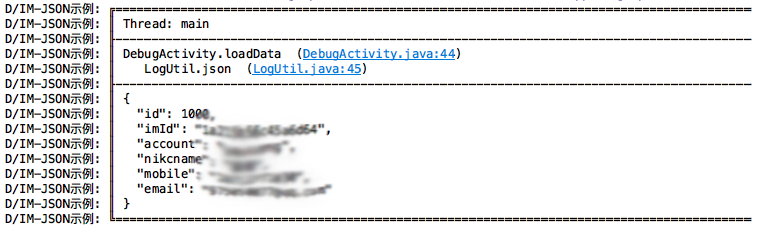
\includegraphics[width=0.95\textwidth]{images/log_sample}
    	\caption{日志信息示例}
    	\label{img_log_sample}
    \end{figure}
    
    
   	\subsubsection{工具库集合的实现}
    

  	\subsection{存储层详细设计与实现}


	
  	\subsection{共识层详细设计与实现}


        

  \subsection{客户端层详细设计与实现}
  	
		\subsubsection{API 客户端服务平台的实现}
		
		
		\subsubsection{gRPC API客户端的实现}
		
		
	 	\subsubsection{RESTful API客户端的实现}
	 	
	 	
		\subsubsection{CLI 命令行客户端的实现}
		


	\subsection{本章小结}
 \clearpage